% Options for packages loaded elsewhere
\PassOptionsToPackage{unicode}{hyperref}
\PassOptionsToPackage{hyphens}{url}
%
\documentclass[
  a4paper,
]{article}
\usepackage{amsmath,amssymb}
\usepackage{setspace}
\usepackage{iftex}
\ifPDFTeX
  \usepackage[T1]{fontenc}
  \usepackage[utf8]{inputenc}
  \usepackage{textcomp} % provide euro and other symbols
\else % if luatex or xetex
  \usepackage{unicode-math} % this also loads fontspec
  \defaultfontfeatures{Scale=MatchLowercase}
  \defaultfontfeatures[\rmfamily]{Ligatures=TeX,Scale=1}
\fi
\usepackage{lmodern}
\ifPDFTeX\else
  % xetex/luatex font selection
\fi
% Use upquote if available, for straight quotes in verbatim environments
\IfFileExists{upquote.sty}{\usepackage{upquote}}{}
\IfFileExists{microtype.sty}{% use microtype if available
  \usepackage[]{microtype}
  \UseMicrotypeSet[protrusion]{basicmath} % disable protrusion for tt fonts
}{}
\makeatletter
\@ifundefined{KOMAClassName}{% if non-KOMA class
  \IfFileExists{parskip.sty}{%
    \usepackage{parskip}
  }{% else
    \setlength{\parindent}{0pt}
    \setlength{\parskip}{6pt plus 2pt minus 1pt}}
}{% if KOMA class
  \KOMAoptions{parskip=half}}
\makeatother
\usepackage{xcolor}
\usepackage[margin=1in]{geometry}
\usepackage{color}
\usepackage{fancyvrb}
\newcommand{\VerbBar}{|}
\newcommand{\VERB}{\Verb[commandchars=\\\{\}]}
\DefineVerbatimEnvironment{Highlighting}{Verbatim}{commandchars=\\\{\}}
% Add ',fontsize=\small' for more characters per line
\usepackage{framed}
\definecolor{shadecolor}{RGB}{248,248,248}
\newenvironment{Shaded}{\begin{snugshade}}{\end{snugshade}}
\newcommand{\AlertTok}[1]{\textcolor[rgb]{0.94,0.16,0.16}{#1}}
\newcommand{\AnnotationTok}[1]{\textcolor[rgb]{0.56,0.35,0.01}{\textbf{\textit{#1}}}}
\newcommand{\AttributeTok}[1]{\textcolor[rgb]{0.13,0.29,0.53}{#1}}
\newcommand{\BaseNTok}[1]{\textcolor[rgb]{0.00,0.00,0.81}{#1}}
\newcommand{\BuiltInTok}[1]{#1}
\newcommand{\CharTok}[1]{\textcolor[rgb]{0.31,0.60,0.02}{#1}}
\newcommand{\CommentTok}[1]{\textcolor[rgb]{0.56,0.35,0.01}{\textit{#1}}}
\newcommand{\CommentVarTok}[1]{\textcolor[rgb]{0.56,0.35,0.01}{\textbf{\textit{#1}}}}
\newcommand{\ConstantTok}[1]{\textcolor[rgb]{0.56,0.35,0.01}{#1}}
\newcommand{\ControlFlowTok}[1]{\textcolor[rgb]{0.13,0.29,0.53}{\textbf{#1}}}
\newcommand{\DataTypeTok}[1]{\textcolor[rgb]{0.13,0.29,0.53}{#1}}
\newcommand{\DecValTok}[1]{\textcolor[rgb]{0.00,0.00,0.81}{#1}}
\newcommand{\DocumentationTok}[1]{\textcolor[rgb]{0.56,0.35,0.01}{\textbf{\textit{#1}}}}
\newcommand{\ErrorTok}[1]{\textcolor[rgb]{0.64,0.00,0.00}{\textbf{#1}}}
\newcommand{\ExtensionTok}[1]{#1}
\newcommand{\FloatTok}[1]{\textcolor[rgb]{0.00,0.00,0.81}{#1}}
\newcommand{\FunctionTok}[1]{\textcolor[rgb]{0.13,0.29,0.53}{\textbf{#1}}}
\newcommand{\ImportTok}[1]{#1}
\newcommand{\InformationTok}[1]{\textcolor[rgb]{0.56,0.35,0.01}{\textbf{\textit{#1}}}}
\newcommand{\KeywordTok}[1]{\textcolor[rgb]{0.13,0.29,0.53}{\textbf{#1}}}
\newcommand{\NormalTok}[1]{#1}
\newcommand{\OperatorTok}[1]{\textcolor[rgb]{0.81,0.36,0.00}{\textbf{#1}}}
\newcommand{\OtherTok}[1]{\textcolor[rgb]{0.56,0.35,0.01}{#1}}
\newcommand{\PreprocessorTok}[1]{\textcolor[rgb]{0.56,0.35,0.01}{\textit{#1}}}
\newcommand{\RegionMarkerTok}[1]{#1}
\newcommand{\SpecialCharTok}[1]{\textcolor[rgb]{0.81,0.36,0.00}{\textbf{#1}}}
\newcommand{\SpecialStringTok}[1]{\textcolor[rgb]{0.31,0.60,0.02}{#1}}
\newcommand{\StringTok}[1]{\textcolor[rgb]{0.31,0.60,0.02}{#1}}
\newcommand{\VariableTok}[1]{\textcolor[rgb]{0.00,0.00,0.00}{#1}}
\newcommand{\VerbatimStringTok}[1]{\textcolor[rgb]{0.31,0.60,0.02}{#1}}
\newcommand{\WarningTok}[1]{\textcolor[rgb]{0.56,0.35,0.01}{\textbf{\textit{#1}}}}
\usepackage{graphicx}
\makeatletter
\def\maxwidth{\ifdim\Gin@nat@width>\linewidth\linewidth\else\Gin@nat@width\fi}
\def\maxheight{\ifdim\Gin@nat@height>\textheight\textheight\else\Gin@nat@height\fi}
\makeatother
% Scale images if necessary, so that they will not overflow the page
% margins by default, and it is still possible to overwrite the defaults
% using explicit options in \includegraphics[width, height, ...]{}
\setkeys{Gin}{width=\maxwidth,height=\maxheight,keepaspectratio}
% Set default figure placement to htbp
\makeatletter
\def\fps@figure{htbp}
\makeatother
\setlength{\emergencystretch}{3em} % prevent overfull lines
\providecommand{\tightlist}{%
  \setlength{\itemsep}{0pt}\setlength{\parskip}{0pt}}
\setcounter{secnumdepth}{-\maxdimen} % remove section numbering
\ifLuaTeX
  \usepackage{selnolig}  % disable illegal ligatures
\fi
\usepackage{bookmark}
\IfFileExists{xurl.sty}{\usepackage{xurl}}{} % add URL line breaks if available
\urlstyle{same}
\hypersetup{
  pdftitle={U4. WINDOWS SERVER. ADMINISTRACIÓ I CONFIGURACIÓ},
  hidelinks,
  pdfcreator={LaTeX via pandoc}}

\title{U4. WINDOWS SERVER. ADMINISTRACIÓ I CONFIGURACIÓ}
\usepackage{etoolbox}
\makeatletter
\providecommand{\subtitle}[1]{% add subtitle to \maketitle
  \apptocmd{\@title}{\par {\large #1 \par}}{}{}
}
\makeatother
\subtitle{COMPARTICIÓ de DIRECTORIS (SHARING) I ASSIGNACIÓ D'UNITATS}
\author{}
\date{\vspace{-2.5em}}

\begin{document}
\maketitle

{
\setcounter{tocdepth}{2}
\tableofcontents
}
\setstretch{1.5}
\renewcommand\tablename{Tabla}
\newpage

\section{RESUM}\label{resum}

Aquest és un tema pont entre la Unitat 3 i la Unitat 4 de la Programació
Didàctica recentement presentada del curs 2024/2025.

Repassem punts avançats sobre la compartició de carpetes en Windows i
els contextualitzem en Unitat Organitzatives introduint el concepte de
``permís efectiu'' que vorem quan tractem els permisos NTFS.

La Unitat 4 tracta el Sistema de Fitxers des de les tres vesssants de la
tríada de la seguretat:

\begin{itemize}
\item
  La \textbf{disponibilitat i confidencialitat}: Permisos efectius i
  quotes.
\item
  La \textbf{integritat}: Directives de seguretat, Backups i RAIDs
\end{itemize}

\section{1 COMPARTICIÓ de CARPETA
(SHARE)}\label{comparticiuxf3-de-carpeta-share}

Ja hem vist la compartició de les carpetes en xarxes Windows, tant en la
part final del curs passat com en les activitats anteriors de Workgroup
i Domini. Podem dir que, junt a la gestió centralitzada de comptes
(usuaris i grups) és el més bàsic d'una xarxa local.

\subsection{1.1 Prèvia}\label{pruxe8via}

En Windows tenim dos sistemes de permisos:

\begin{itemize}
\item
  Sharing o compartició de carpetes. Admet només permisos de Lectura,
  Escriptura i Control Total. Poden aplicarse sobre particions NTFS o
  FAT32. S'apliquen només si accedim per la xarxa.
\item
  Permisos NTFS, permet detallar més les accions a poder fer en el
  sistema de fitxers. En un domini, el normal és aplicar-los després de
  l'anterior per concretar el permisos. Només s'apliquen sobre
  particions NTFS i actuen també en local.
\end{itemize}

Anem a centrar-nos en els permisos SHARE

\subsection{1.2 Permisos de Compartició
(Sharing)}\label{permisos-de-comparticiuxf3-sharing}

Els permisos de \textbf{compartició (sharing)} en Windows es configuren
per controlar l'accés a carpetes \textbf{a través de la xarxa}, sense
alterar els permisos NTFS locals.

Els permisos de compartició són més simples que els NTFS i es centren
principalment en el nivell d'accés remot, mentre que la
\textbf{propietat} fa referència a qui és el responsable de la carpeta o
fitxer, la qual cosa afecta la capacitat de gestió de permisos.

Els permisos de compartició s'utilitzen tres tipus principals:

\textbf{Lectura (Read)}: Permet veure el contingut de la carpeta i obrir
fitxers, però no es poden modificar ni crear nous elements.

\textbf{Canvi (Change)}: A banda de lectura, permet modificar (editar,
afegir i eliminar fitxers o carpetes) dins de la carpeta compartida.

\textbf{Control total (Full Control)}: Dóna al usuari o grup el màxim
nivell d'accés. A bada dels anteriors, canviar els permisos de
compartició de la carpeta.

\begin{quote}
\textbf{Nota:} Es tracta de decidir quins grups/usuaria accediran des de
la xarxa i què podran fer.
\end{quote}

\subsection{1.3 La propietat}\label{la-propietat}

Només el \textbf{propietari} (o un administrador) té permisos per
ajustar els permisos de compartició (i NTFS de la carpeta). La propietat
també permet que el propietari puga recuperar l'accés o modificar
permisos, fins i tot si altres usuaris han establert restriccions.

\begin{center}\rule{0.5\linewidth}{0.5pt}\end{center}

\section{2. CONFIGURACIÓ}\label{configuraciuxf3}

Els passos generals són:

\begin{enumerate}
\def\labelenumi{\arabic{enumi}.}
\item
  \textbf{Seleccionar la carpeta}: Clic dret a la carpeta que vols
  compartir i seleccionar \textbf{Propietats}.
\item
  \textbf{Compartició}: Accedir a la pestanya \textbf{Compartició} i fer
  clic a \textbf{Compartir\ldots{}} o \textbf{Compartició avançada} per
  opcions més detallades.
\item
  \textbf{Afegeix usuaris}: En aquesta finestra, pots especificar grups
  o usuaris concrets de la xarxa (locals del Servidor no té cap sentit)
  i assignar els permisos adequats (Lectura, Canvi o Control total).
\item
  \textbf{Guardar canvis}: Recordeu que heu de provar accedint des de
  Xarxa. No a c:/... d:/...
\end{enumerate}

\subsection{\texorpdfstring{2.1 Herència i Permisos Efectius en
Compartició \emph{( ho vorem de nou en donar
NTFS)}}{2.1 Herència i Permisos Efectius en Compartició ( ho vorem de nou en donar NTFS)}}\label{heruxe8ncia-i-permisos-efectius-en-comparticiuxf3-ho-vorem-de-nou-en-donar-ntfs}

Els permisos de compartició no tenen herència (NTFS, sí).
\textbf{S'apliquen només a la carpeta compartida i no a les
subcarpetes}. No obstant vorem més avant que els \textbf{permisos
efectius} en una carpeta compartida són la combinació dels dos tipus de
permisos amb regles en cas de contradicció.

\subsection{2.2 Recomanacions}\label{recomanacions}

\begin{itemize}
\item
  \textbf{Assigna permisos mínims}: Com sempre, limita l'accés de cada
  grup als permisos mínims que necessite (Lectura/Canvi/Control total)
  per minimitzar riscos de seguretat. \textbf{Evita ``Control total''}.
\item
  \textbf{Revisa els permisos efectius} per garantir que els usuaris
  només tinguin l'accés necessari quan combinen permisos de compartició
  amb els permisos NTFS locals.
\item
  \textbf{Crea grups} encara que siga d'un usuari, et facilitarà la
  gestió si després tens nous usuaris de perfils similar.
\end{itemize}

\begin{center}\rule{0.5\linewidth}{0.5pt}\end{center}

\section{3 OPERATIVA}\label{operativa}

\subsection{3.1 Compartició}\label{comparticiuxf3}

Des del Servidor compartim unes carpetes.

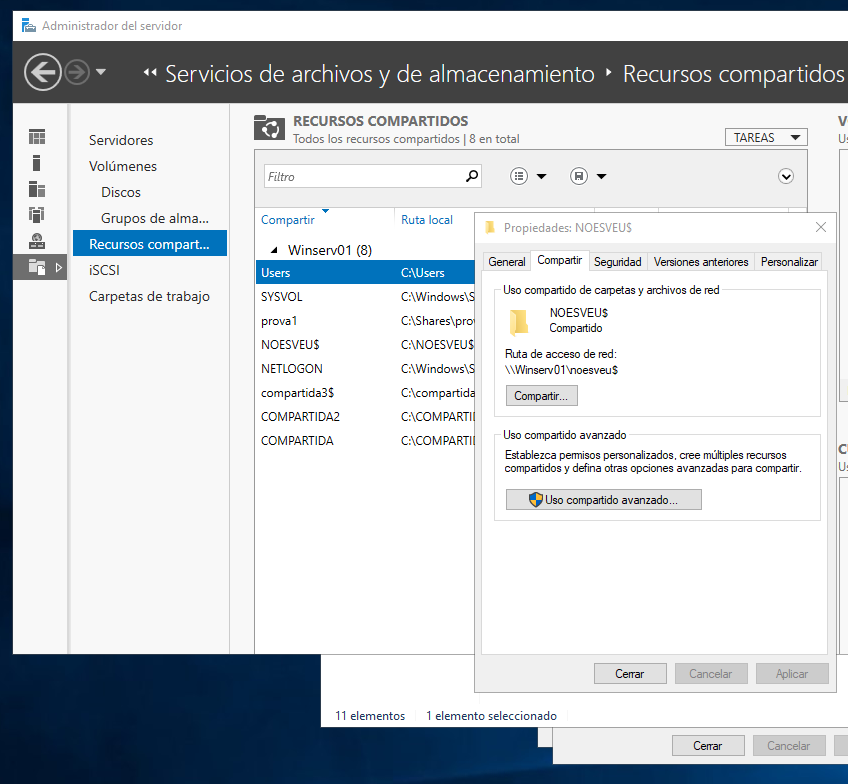
\includegraphics{png/CarpetesCompartides1.png}
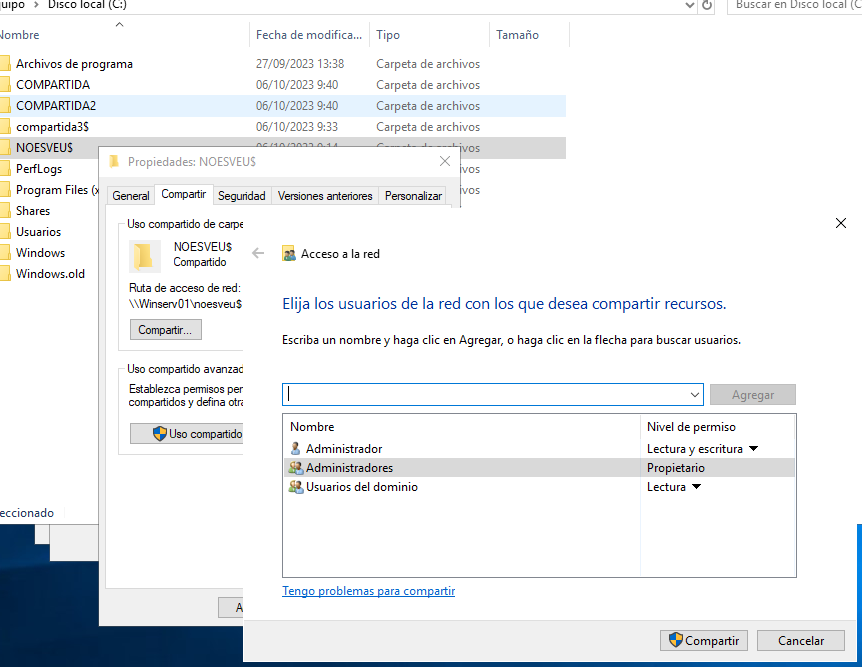
\includegraphics{png/CarpetesCompartides2.png}

Podeu usar la consola \textbf{fsmgmt.msc} de CARPETES COMPARTIDES per
crear, compartir i assignar permisos NTFS.

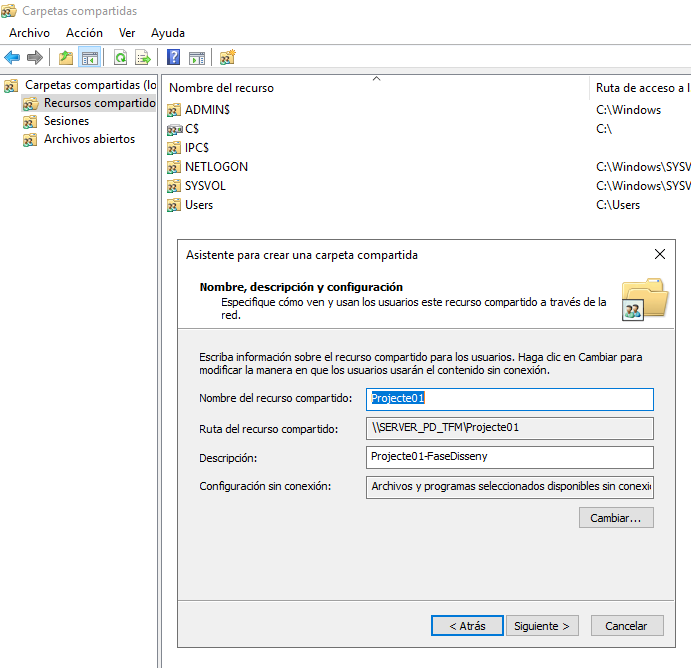
\includegraphics{png/CC1.png}

\subsection{3.2 Compartició avançada}\label{comparticiuxf3-avanuxe7ada}

\begin{itemize}
\item
  CONTROL TOTAL Permís per a canviar el permisos i propietari.
\item
  NOMBRE D'ACCESOS PERMESOS podem limitar la quantitat d'usuaris de la
  xarxa que poden accedir al mateix temps.
\item
  NOM DEL RECURS COMPARTIT Si volem que la carpeta es veja a la xarxa
  amb un altre nom.
\end{itemize}

\includegraphics{png/usCompartitAvançat.png}
\includegraphics{png/usCompartitAvançat2.png}
\includegraphics{png/usCompartitAvançat3.png}

Recordeu que en la consola \textbf{fsmgmt.msc} veieu les sessions de
xarxa. Si s'ha superat el \textbf{nombre màxim d'accessos simultanis} a
una carpeta, podeu consultar (i expulsar l'usuari des d'ací).

\begin{center}\rule{0.5\linewidth}{0.5pt}\end{center}

\section{4 ACCESOS I MAPEIG}\label{accesos-i-mapeig}

Des del client podem accedir als primers recursos compartits fins i tot
si estan ocults

\subsection{4.1 Formes d'accedir}\label{formes-daccedir}

Si observem, podem vore les carpetes des de Red del client ( Windows 1x
) de 4 formes.

\begin{itemize}
\item
  Gràficament des de l'explorador buscant el servidor
\item
  Gràficament des de l'explorador amb la IP del servidor. Útil per a:

  \begin{itemize}
  \item
    Descatar si falla la resolució de noms per provar però no la
    connexió a nivell de xarxa.
  \item
    Visualitzar els directoris ocults escrivint el nom de recurs
    compartit amb el \$
  \end{itemize}
\item
  Des de l'interface d'ordres amb NET SHARE.
\item
  Des de Powershell.
\end{itemize}

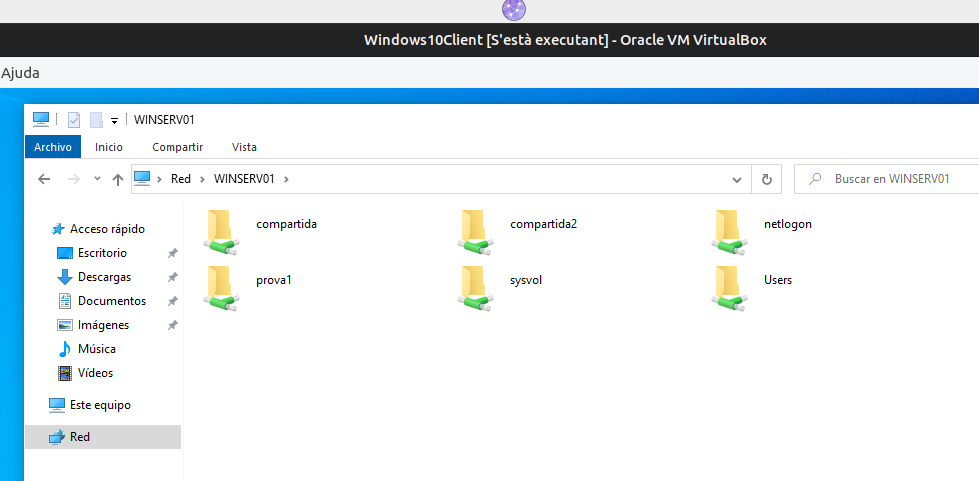
\includegraphics{png/CarpetesCompartidesDesdeWin10.png}
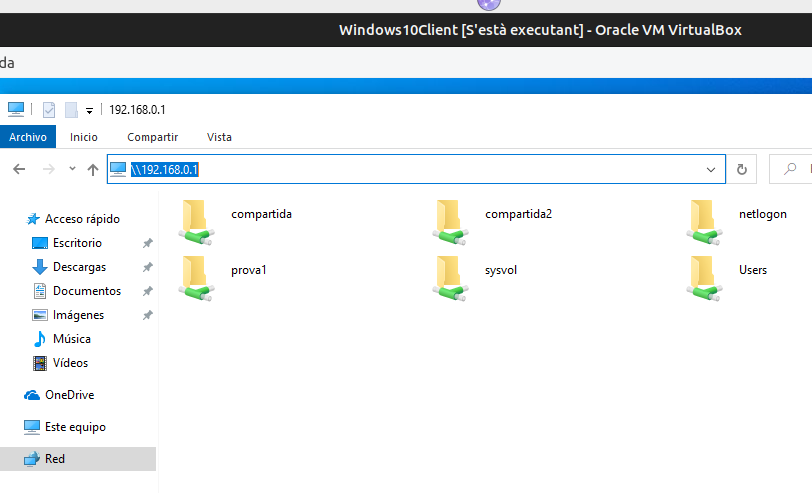
\includegraphics{png/CarpetesCompartidesDesdeWin10IP.png}
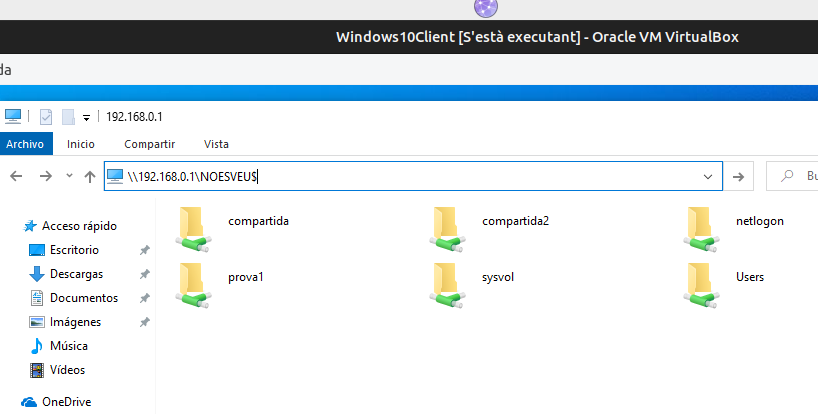
\includegraphics{png/CarpetesCompartidesOcultesDesdeWin10.png}

L'assignació d'unitats es pot fer des del

\begin{itemize}
\tightlist
\item
  GUI.
\item
  Des del cmd (\emph{net use}, com ja vam avançar)*.
\item
  PowerShell. Teniu informació al Repositori de PowerShell
\item
  Carpetes Particulars (ja estudiat).
\item
  GPO (apartat següent)
\end{itemize}

Teniu informació sobre com s'accedeix amb els cdmLets de PowerShell al
repositori de PowerShell:

\href{https://github.com/tofermos/PowerShell/blob/main/md/PSCompartirRecursos.md}{Repositori
PowerShell}

\begin{quote}
TERMES QUIVALENTS: Assignar unitat de xarxa, mapeig, capturar
unitat\ldots{} és el mateix.
\end{quote}

\section{5 RELACIÓ AMB LES UNITATS ORGANITZATIVES i
DIRECTIVA}\label{relaciuxf3-amb-les-unitats-organitzatives-i-directiva}

És molt probable que ens interesse que un departament o una delegació de
d l'empresa (una part del domini), els grups accedisquen a unes
determindaes carpetes. I que tots accedisquen igual. Amb el que hem vist
al tema de UO i en aquest, podem donar solució. Fent que les carpetes
estiguen a la UO i, amb la directiva, tots esl usuaris de la UO
accedisquen igual (F:, per exemple)

\subsection{5.1 Mapeig per GPO}\label{mapeig-per-gpo}

L'assignació d'una unitat de xarxa mitjançant una \textbf{Directiva de
Grup (Group Policy Object, GPO)}, és centralitzat per al Domoini o UO
amb tots els avantatges importants de seguretat i administració que
comporta.

Avantatges:

\begin{enumerate}
\def\labelenumi{\arabic{enumi}.}
\item
  \textbf{Control Centralitzat d'Accés}
\item
  \textbf{Assignació Automàtica amb Seguretat}: En lloc de confiar que
  cada usuari faci el mapeig manualment amb errors possibles.
\item
  \textbf{Opcions de Filtrat per Seguretat}: A les GPOs pots fer ús del
  filtrat de seguretat i la \textbf{delimitació per grups}.
\item
  \textbf{Opcions de Reconnectivitat i Persistència}: Les GPOs permeten
  definir si la unitat s'ha de tornar a connectar en iniciar sessió o
  no.
\item
  \textbf{Auditoria i Compliment}: Mitjançant registres d'auditoria a
  l'Active Directory, pots seguir qui ha accedit als recursos
  compartits.
\end{enumerate}

\subsection{5.2 Operativa}\label{operativa-1}

\begin{enumerate}
\def\labelenumi{\arabic{enumi}.}
\tightlist
\item
  **Obre la Consola de Gestió de Directives de Grup (gpmc.msc)
\item
  Crea o selecciona una GPO existent en el domini o unitat organitzativa
  (OU) a la qual vols el mapeig.
\item
  Ves a: \textbf{Configuració d'Usuari} \textgreater{}
  \textbf{Preferències} \textgreater{} \textbf{Configuració de Windows}
  \textgreater{} \textbf{Unitats}.
\item
  Fes clic amb el botó dret i selecciona \textbf{Nuevo} \textgreater{}
  \textbf{Unitat de Mapeig}.
\item
  Indica lletra disponible i del recurs compartit (per exemple,
  \texttt{\textbackslash{}\textbackslash{}WindowsServerDC\textbackslash{}NotesTakeHome}).
\item
  Selecciona les opcions d'actualització, connexió i desconnexió segons
  els requisits de seguretat i persistència.
\item
  Utilitza el \textbf{Filtrat de Seguretat} per aplicar la GPO només a
  grups específics si cal.
\end{enumerate}

\begin{figure}
\centering
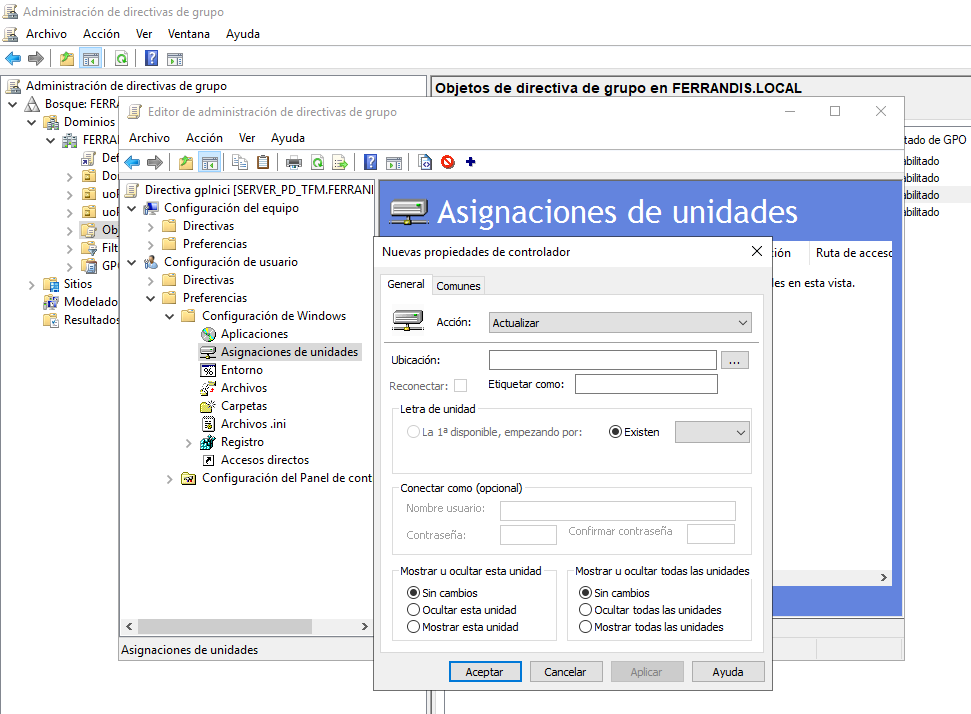
\includegraphics{png/CapturaGPO.png}
\caption{GPO Assignació Unitat}
\end{figure}

Recorda:

\begin{Shaded}
\begin{Highlighting}[]
\NormalTok{gpupdate }\AttributeTok{/force}
\end{Highlighting}
\end{Shaded}


\end{document}
